%%%%%%%%%共通の設定%%%%%%%%
\documentclass[14pt]{ltjsarticle}
\usepackage{mathtools}%数学論文用マクロであるamsmathの拡張
\usepackage{amssymb}%AMSFonts
\usepackage{bm}%イタリック体の太字
\usepackage{mathrsfs}%RSFSフォント,花文字
%複数行コメントアウト
\usepackage{comment}
  \includecomment{uncomment}\excludecomment{encomment}
\usepackage{ascmac}%別行立てで文章を囲む
%図
\usepackage{tikz}
  \usetikzlibrary{arrows.meta}
  \usetikzlibrary{shapes.geometric}
  \usetikzlibrary {shapes.misc}
  \usetikzlibrary{positioning}
%----%\usepackage{otf}%強調コマンドを再定義,入れ子も可能%%%%%%%%%%%%%%%%%%%%%%%%%%%%%%%%%%%%%%%%%%%%%%%%pLaTeX2eが要求される%%
%----%  \DeclareEmphSequence{\bfseries\gtfamily, \sffamily\mcfamily}
%ソースコード環境
\usepackage{listings,jvlisting}
  %ソースコードの表示に関する設定
  \lstset{% 
    language={Scala}, 
    backgroundcolor={\color[gray]{.85}},% 
    basicstyle={\small},% 
    identifierstyle={\small},% 
    commentstyle={\small\ttfamily \color[rgb]{0,0.5,0}},% 
    keywordstyle={\small\bfseries \color[rgb]{0,0,1}},% 
    ndkeywordstyle={\small},% 
    stringstyle={\small\ttfamily}, 
    frame={tb}, 
    breaklines=true, 
    columns=[l]{fullflexible},% 
    numbers=left,% 
    xrightmargin=0\zw,% 
    xleftmargin=3\zw,% 
    numberstyle={\scriptsize},% 
    stepnumber=1, 
    numbersep=1\zw,% 
    morecomment=[l]{//}% 
  }
  \renewcommand{\lstlistingname}{ソースコード}%listingnameの変更
%数学マクロ  
\newcommand{\N}{\mathbb{N}}%自然数全体
\newcommand{\Z}{\mathbb{Z}}%有理整数環
\newcommand{\Q}{\mathbb{Q}}%有理数体
\newcommand{\R}{\mathbb{R}}%実数体
\newcommand{\C}{\mathbb{C}}%複素数体
\newcommand{\p}{\mathcal{P}}%冪
\renewcommand{\o}{\mathcal{O}}%開集合族
\renewcommand{\u}{\mathcal{U}}%宇宙
%自分用の書き換え
\renewcommand{\epsilon}{\varepsilon}
\renewcommand{\phi}{\varphi}
\renewcommand{\subset}{\subseteq}
%数学マクロ
\newcommand{\set}[1]{\{\,#1\,\}}%\midや;を用いる
\newcommand{\map}[3]{#1\colon#2\longrightarrow#3}
\newcommand{\Map}[2]{#1\stackrel{#2}{\longrightarrow}}%domainとarrowのみ
\newcommand{\pair}[1]{\langle#1\rangle}%山括弧
\newcommand{\note}[1]{\quad(\,#1\,)}%補足
%一般マクロ
%%%%%%%%%%%特定の設定%%%%%%%%%%%%
%headerとfooter
\usepackage{fancyhdr}
  \pagestyle{fancy}
  \rhead{header right}
  \cfoot{\thepage}
%タイトル
\title{
  Title
    \large{\\---Subtitle---}
}
\author{Author\footnote{belong to A} }
\date{\today}
%見出しの変更
\renewcommand{\thesection}{\arabic{section}}
\renewcommand{\thesubsection}{\arabic{subsection}}
%enumeitemの変更
\usepackage{enumitem}
  \setlist[enumerate, 1]{label=(\theenumi)}
  \setlist[itemize, 1]{label=・}
%ハイパーリンクの設定
\usepackage{color, hyperref}
  \usepackage{url}
  \usepackage{xcolor}
  \hypersetup{
      colorlinks=true,
      citecolor=blue,
      linkcolor=red,
      urlcolor=orange,
  }
%定理環境
\usepackage{amsthm}
  \theoremstyle{definition}
  \newtheorem{thm}{定理}
  \newtheorem{dfn}[thm]{定義}
  \newtheorem{prop}[thm]{命題}
  \newtheorem{lem}[thm]{補題}
  \newtheorem{cor}[thm]{系}
  \newtheorem{cf}[thm]{例}
  \newtheorem{rem}[thm]{注意}
  \newtheorem{ex}[thm]{問題}
  \newtheorem{axm}[thm]{公理}
  \numberwithin{thm}{section}
%数学マクロ
\DeclareMathOperator{\Ob}{Ob}
\DeclareMathOperator{\Mor}{Mor}
\DeclareMathOperator{\dom}{dom}
\DeclareMathOperator{\cod}{cod}
\DeclareMathOperator{\Hom}{Hom}
\DeclareMathOperator{\id}{id}
\DeclareMathOperator{\Lim}{Lim}
\DeclareMathOperator{\Colim}{Colim}
\renewcommand{\c}{\mathscr{C}}%圏
\renewcommand{\d}{\mathscr{D}}
\newcommand{\I}{\mathbf{I}}%添字圏
\renewcommand{\j}{\mathscr{J}}
\newcommand{\Set}{\mathbf{Set}}
\newcommand{\Vect}{\mathbf{Vect}}
\newcommand{\Mod}{\mathbf{Mod}}
\newcommand{\Pos}{\mathbf{Pos}}
\newcommand{\Grp}{\mathbf{Grp}}
\newcommand{\Cat}{\mathbf{Cat}}
\newcommand{\Id}{\mathrm{Id}}%関手
\newcommand{\op}{\mathrm{op}}%双対
\newcommand{\placeholder}{{-}}%扱いをマイナス記号と区別
\newcommand{\yoneda}{\mbox{よ}}%米田埋込
\newcommand{\yoyoneda}{\mbox{ね}}%余米田埋込
%一般マクロ
\newcommand{\head}[1]{\overset{\downarrow}{#1}}
%開発中の設定
\begin{uncomment}
  \usepackage{silence}%煩わしいwarningをignore
    \WarningFilter{latexfont}{Font shape}
    \WarningFilter{latexfont}{Size substitutions}
\end{uncomment}
% shortcut in VScode
% cmd + s                               save (and build)
% cmd + opt + b                         build
% cmd + opt + v                         open viewer
% cmd + opt + j                         TeX -> PDF
% move cursor on viewer, cmd + click    PDF -> TeX
% Shift + ctrl + @                      open terminal tab (Problem etc.)
\begin{document}
\maketitle
\thispagestyle{plain}%titleのpagestyleはデフォルトに戻るため,独立に設定

\begin{abstract}
  Abstract.
\end{abstract}

\newpage
\section{Section1}

\begin{itembox}[l]{CWM}
  All consepts are Kan extensions.
\end{itembox}

\begin{dfn}
  \emph{The Term}(term)$T$ consists of
  \begin{enumerate}
    \item T1,
    \item T2,
    \item T3,
  \end{enumerate}
  and is satisfied from
  \begin{enumerate}[resume]
    \item \emph{laws1},
    \item \emph{laws2}.
  \end{enumerate}
\end{dfn}

\begin{rem}
  Please reference Maclane \cite{マックレーン}.
\end{rem}

\begin{cf}
  Examples are the following table :
  \begin{flushleft}
    \begin{tabular}{ll}
      $A$ &
      Apple \\
      $B$ &
      Bird  \\
      $C$ &
      Cat   \\
      $D$ &
      Dog
    \end{tabular}
  \end{flushleft}
\end{cf}

\section{Section2}

\begin{dfn}
  \[
    \Hom_\c(A,B)\ni f\longmapsto Ff\in\Hom_\d(FA,FB)
  \]
\end{dfn}

\begin{prop}
  A Proposition.
\end{prop}

\begin{proof}
  \[
    h\circ Ff=\id_{FA}
    \iff F(gf)=F(\id_A)
    \iff gf=\id_A.
  \]
\end{proof}

\begin{cor}\label{cor1}
  \[
    A\cong B\text{ならば}FA\cong FB.
  \]
\end{cor}

\section{Section3}

\section{Section4}

\begin{thm}[Yoneda Lemma]
  \[
    \Hom_{\widehat{\c}}(\Hom_\c(-,C),P)\cong PC.
  \]
\end{thm}

\begin{proof}
  That's true.
  \begin{center}%自然変換の図式
    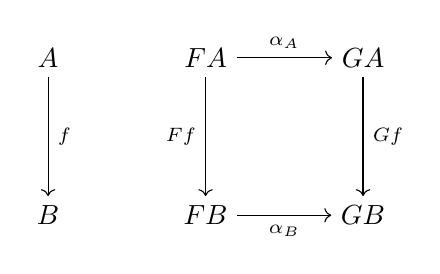
\begin{tikzpicture}[auto]
      \node (a) at (-2,2) {$A$};
      \node (b) at (-2,0) {$B$};

      \node (Fa) at (0,2) {$FA$}; \node (Ga) at (2,2) {$GA$};
      \node (Fb) at (0,0) {$FB$}; \node (Gb) at (2,0) {$GB$};

      \draw[->] (a) to node {$\scriptstyle f$} (b);

      \draw[->] (Fa) to node {$\scriptstyle \alpha_A$} (Ga);
      \draw[->] (Ga) to node {$\scriptstyle Gf$} (Gb);

      \draw[->] (Fa) to node[swap] {$\scriptstyle Ff$} (Fb);
      \draw[->] (Fb) to node[swap] {$\scriptstyle \alpha_B$} (Gb);
    \end{tikzpicture}
  \end{center}
\end{proof}

\[
  \Hom_\c(C,C')\cong\Hom_{\widehat{\c}}
  (\Hom_\c(-,C),\Hom_\c(-,C')).
\]

\begin{cor}\label{cor2}
  \[
    \Hom_\c(-,A)\cong\Hom_\c(-,B)\iff A\cong B.
  \]
\end{cor}

\section{section5}
与えられた疑似コードのフローチャートは図\ref{flow}の通りであり,
アセンブリ言語によるプログラムは表\ref{program1}の通りである.
\begin{figure}[ht]
  \caption{フローチャート}
  \label{flow}
  \centering
  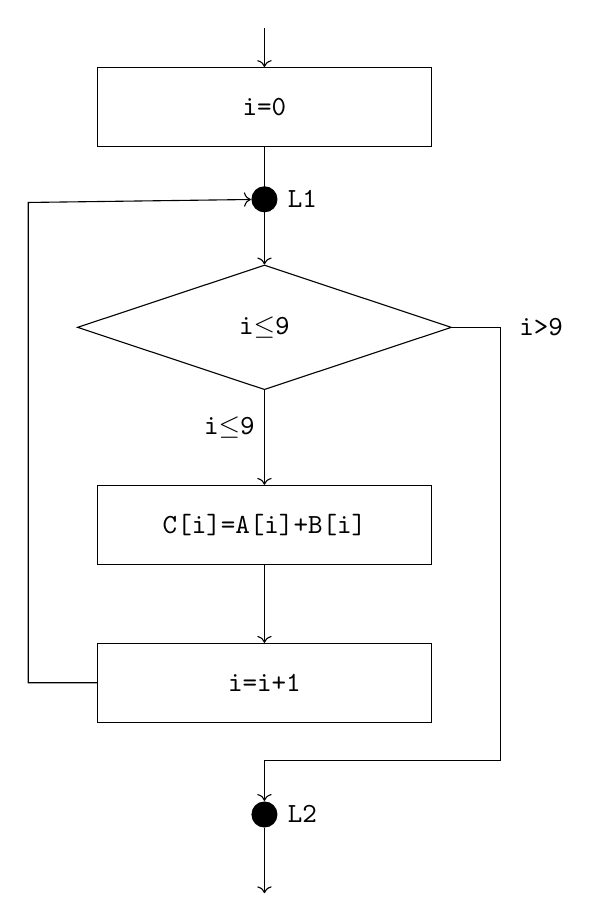
\begin{tikzpicture}
    \tikzset{Terminal/.style={rounded rectangle,  draw,  text centered, text width=3cm, minimum height=1cm}};
    \tikzset{Process/.style={rectangle,  draw,  text centered, text width=4cm, minimum height=1cm}};
    \tikzset{Decision/.style={diamond,  draw,  text centered, aspect=3,text width=3cm, minimum height=1cm}};
    \tikzset{Point/.style={circle, fill}}

    \node[Process](a)at (0,0){\texttt{i=0}};
    \node[Point, below=1 of a.center, label=right:\texttt{L1}] (p) {};
    \node[Decision, below=2 of a.center](b){\texttt{i$\leq$9}};
    \node[Process, below=2 of b.center](c){\texttt{C[i]=A[i]+B[i]}};
    \node[Process, below=1.5 of c.center](d){\texttt{i=i+1}};
    \node[Point, below=1.5 of d.center, label=right:\texttt{L2}] (q) {};

    \draw[<-] (a) --+(0, 1);
    \draw[->] (a) --(b);
    \draw[->] (b) --(c) node[left, yshift=35] {\texttt{i$\leq$9}};
    \draw[->] (c) --(d);

    \draw[->] (d) --++(-3, 0)--++(0, 6.1)--(p);
    \draw[->] (b) node[xshift=100] {\texttt{i>9}}
    --++(3, 0)--++(0, -5.5)--++(-3, 0)--(q);

    \draw[->] (q) --+(0, -1);
  \end{tikzpicture}
\end{figure}

\begin{table}[ht]
  \caption{プログラム}
  \label{program1}
  \centering
  \begin{tabular}{lllll}
                    & LD\qquad\qquad\qquad\qquad & GR4, & ZERO &     \\
    L1:\qquad\qquad & CPA                        & GR4, & NINE &     \\
                    & JPL                        & L2   &      &     \\
                    & LD                         & GR3, & A,   & GR4 \\
                    & ADDA                       & GR3, & B,   & GR4 \\
                    & ST                         & GR3, & C,   & GR4 \\
                    & ADDA                       & GR4, & ONE  &     \\
                    & JUMP                       & L1   &      &     \\
    L2:             & (次の命令)                     &      &      &
  \end{tabular}
\end{table}

アルゴリズム「Minimum」を実現する疑似コードはソースコード\ref{min}の通りである.
\newpage
\begin{lstlisting}[caption=Minimum,label=min]
t = B[0];
for(i = 1; i < n; i++){
  if(B[i] < t){
    t = B[i];
  }
}
  \end{lstlisting}

\section{section6}
圏\(\c\)上の\emph{米田埋込},\emph{余米田埋込}をそれぞれ
\[
  \map{{}^{\c}\yoneda}{\c}{\widehat{\c}},\quad\map{{}^{\c}\yoyoneda}{\c^{\op}}{\widehat{\c^{\op}}}
\]
と表し,圏\(\c\)が文脈から明らかな場合は,
単に\(\yoneda,\,\yoyoneda\)と表す.
各\(A,B\in\c\)に対して,
\[
  \yoneda(B)=\yoneda^B = \Hom_\c (\placeholder, B),\quad
  \yoyoneda(A) = \yoneda_A = \Hom_\c (A, \placeholder)
\]
と表す.すなわち,\(\yoneda^B(A) = \Hom(A, B) = \yoneda_A(B)\)である.


\begin{thebibliography}{99}
  \bibitem{レンスター} T. レンスター著,土岡俊介訳,「ベーシック圏論」,
  丸善出版,2017.
  \bibitem{マックレーン} S. マックレーン著,三好博之,高木理訳,「圏論の基礎」,
  丸善出版,2012.
  \bibitem{alg-d} 壱大整域 \url{http://alg-d.com/math/kan_extension/}.
\end{thebibliography}
\end{document}